\subsection{Replikasi basis data}

Replikasi berarti menyimpan salinan data yang sama pada beberapa mesin yang berbeda dan terhubung pada jaringan \parencite{dataIntensiveApplications}. Terdapat beberapa alasan mengapa hal ini lazim dilakukan, yaitu:

\begin{enumerate}
    \item Untuk menjaga data tetap dekat secara geografis kepada pengguna, sehingga latensi berkurang.
    \item Agar sistem dapat terus berjalan meski terjadi kegagalan pada sebagian sistem, sehingga menjaga ketersediaan sistem.
    \item Untuk meningkatkan jumlah mesin yang bisa melayani permintaan baca.
\end{enumerate}

Salah satu pendekatan yang umum diimplementasikan pada basis data relasional seperti PostgreSQL adalah replikasi berbasiskan pemimpin (\textit{leader}) dan pengikut (\textit{follower}). Satu \textit{node} ditugaskan sebagai pemimpin yang melayani permintaan baca dan tulis, lalu setiap perubahan yang terjadi akan direplikasi oleh replika (pengikut). Dengan pola seperti ini, umumnya operasi tulis hanya dapat ditangani oleh pemimpin dan operasi baca dapat ditangani oleh semua \textit{node}.

\begin{figure}[htbp]
    \centering
    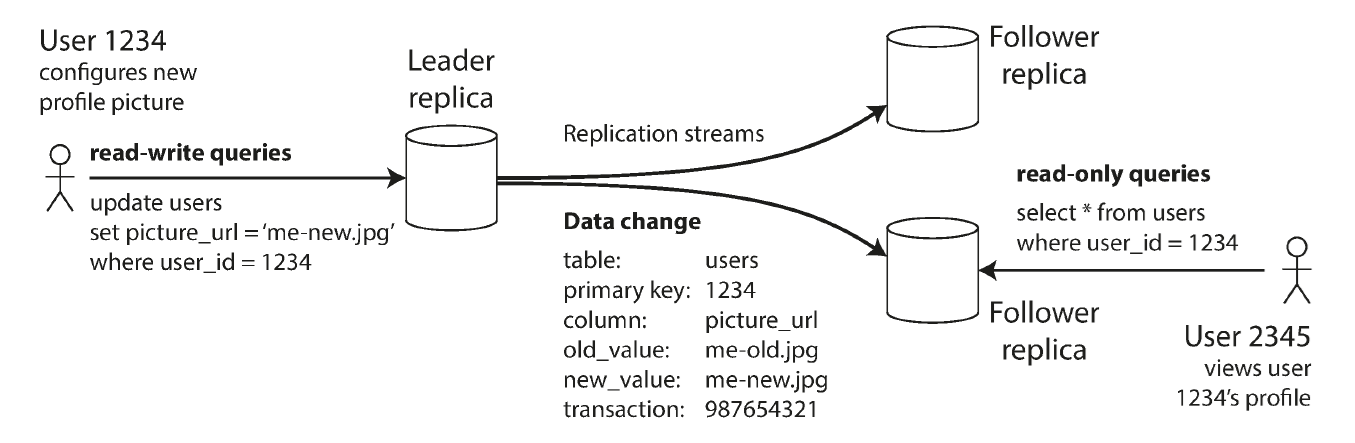
\includegraphics[width=0.8\textwidth]{resources/chapter-2/leader-based-replication.png}
    \caption{Replikasi berdasarkan pemimpin-pengikut \parencite{dataIntensiveApplications}}
    \label{fig:leader-based-replication}
\end{figure}

Selain itu, tipe replikasi juga terbagi menjadi dua, yaitu replikasi sinkron dan replikasi asinkron. Pada replikasi sinkron, data yang akan ditulis harus sudah ditulis oleh semua (atau mayoritas) replika sebelum dapat dianggap sukses. Pada replikasi asinkron, data akan diterima dan ditulis terlebih dahulu pada pemimpin, lalu perubahannya dipropagasikan kepada replika. Setiap pendekatan ini memiliki \textit{tradeoff} tersendiri. Replikasi sinkron menjamin mayoritas \textit{node} memiliki data terbaru, tetapi latensi pada proses penulisan akan meningkat, sedangkan pada replikasi asinkron latensi penulisan jauh lebih kecil, tetapi data pada replika menjadi \textit{eventually consistent}. Kedua tipe replikasi ini didukung oleh PostgreSQL.
